% 論文化方針と結果イメージ（DMDU: RDM・感度分析・DAPP）
% コンパイル: cd docs/paper && latexmk -lualatex paper_plan.tex
% 図の再生成: .venv/bin/python docs/paper/make_figs.py
\documentclass[a4paper,10pt]{ltjsarticle}
\usepackage[margin=22mm]{geometry}
\usepackage{amsmath,amssymb}
\usepackage{graphicx}
\usepackage{booktabs}
\usepackage{multirow}
\usepackage{tabularx}
\usepackage{enumitem}
\usepackage{xcolor}
\usepackage{float}
\usepackage{tikz}
\usetikzlibrary{positioning,arrows.meta,fit}
\usepackage[hidelinks]{hyperref}
\setlist{nosep,leftmargin=1.5em}
\definecolor{cblue}{HTML}{2A78D6}
\definecolor{corange}{HTML}{EB6834}
\definecolor{caqua}{HTML}{1BAF7A}
\definecolor{cgray}{HTML}{52514E}
\newcommand{\todo}[1]{\textcolor{corange}{【#1】}}
\newcommand{\prelim}{\textsuperscript{\textcolor{cgray}{†}}}

\title{気候変動下の流域治水における多主体・深い不確実性下の意思決定\\[2pt]
\large ― 分布型降雨流出氾濫モデルに基づく RDM・大域感度分析・適応経路（DAPP）の統合 ―\\[6pt]
\normalsize 論文化方針と結果イメージ（試行計算に基づく草案）}
\author{}
\date{2026年10月28日}

\begin{document}
\maketitle

\begin{abstract}
本資料は、阿武隈川全域（1000 m メッシュ）を対象に実装した
Robust Decision Making（RDM）、感度分析（Morris・Sobol・意思決定感度・選好感度）、
Dynamic Adaptive Policy Pathways（DAPP）の結果を踏まえ、論文としての主張・構成・図表・本計算計画・
想定される査読上の論点を整理したものである。
掲載する数値と図はすべて \texttt{--quick} 設定の試行計算（RRI 計 約240回）による\textbf{結果イメージ}であり、
本計算（第\ref{sec:plan}節）で置き換える。試行値には\prelim を付す。
\end{abstract}

\tableofcontents
\bigskip

%=====================================================================
\section{論文の主張}
\label{sec:claim}

\subsection{背景と問題設定}
流域治水では、堤防・遊水地といった構造物と、田んぼダム・森林化・住宅の嵩上げや移転といった
流域全体での対策を組み合わせる。組合せの評価には次の三つの難しさがある。
(i) 気候変動の将来像や施策効果に\textbf{深い不確実性}があり、確率分布を合意できない。
(ii) 上流・下流の自治体、国、住民で、便益と費用の帰着先、重視する指標が異なる（\textbf{多主体}）。
(iii) 施策には着手から効果発現までの遅れがあり、気候の変化に合わせて\textbf{いつ}何をするかが問われる。
DMDU（Decision Making under Deep Uncertainty）の研究は多いが、分布型の物理ベース流出氾濫モデルと
資産レベルの被害推計を、多主体の Regret 評価、大域感度分析、適応経路と一貫して接続した例は少ない。
\todo{先行研究レビュー：RDM（Lempert ら）、MORDM（Kasprzyk ら）、DAPP（Haasnoot ら）、
国内の流域治水・田んぼダム評価、RRI の適用例を整理}

\subsection{リサーチクエスチョン}
\begin{description}
\item[RQ1（頑健性と対立）] 予算制約下の流域治水ポートフォリオにおいて、名目シナリオでの最適案と
不確実性下で頑健な案（Minimax Regret）はどの程度異なるか。主体間の対立はどこに生じるか。
\item[RQ2（不確実性の重要度）] 被害額、主体ごとの Regret、施策の選択を支配する不確実性は何か。
気候・降雨パターン・施策効果・費用・選好の寄与を比較する。
\item[RQ3（時間軸）] 気候経路に沿って段階的に投資する場合、どの戦略が頑健か。
適応転換点（ATP）はいつ到来し、観測にもとづく切替は間に合うか。
\end{description}

\subsection{期待される主張（試行結果からの仮説）}
\begin{enumerate}
\item \textbf{名目最適 $\neq$ 頑健}：上流自治体は名目シナリオでは案12 が最良だが、
不確実性下では案10 が 82\%\prelim のサンプルで最良となり、名目最良からの順位逆転率は 88\%\prelim。
\item \textbf{全員を満たす案はない}：すべての主体の許容 Regret（0.05）を同時に満たす案はなかった
（最大 Regret$/$閾値 の最小値 3.4\prelim）。重みを同時にランダム化しても、全主体の推奨案が一致する割合は 0.05\%\prelim。
対立は主に\textbf{費用の帰着}（どの地域の事業費か）と、上流対策の下流への便益から生じる。
\item \textbf{被害は気候、Regret は相互作用}：推奨案の被害額は降雨倍率（$S_T$ 0.63\prelim）と降雨強度分布（0.32\prelim）が支配する。
一方、Regret では $S_T \gg S_1$ で、気候・施策効果・事業費の相互作用が大きい。
施策効果の不確実性は被害額そのものより\textbf{被害軽減量}（田んぼダム効果 $S_T$ 0.24\prelim）に効く。
\item \textbf{段階的投資が頑健、観測トリガーは遅れる}：DAPP では段階的投資が Minimax Regret となった（国・上流自治体）。
観測した被害で切り替える状況適応型は、4℃経路で切替が 2080年\prelim になり ATP（2080年）を回避できない。
気候そのものの観測（降雨倍率）を指標にすること、事前に準備しておくことが必要である。
\end{enumerate}

\subsection{新規性}
\begin{enumerate}
\item 分布型 RRI モデルにセル内標高（サブグリッド）による資産被害と農業被害を組み込み、DMDU の評価器として用いる。
物理過程を変えずに、施策は地形・土地利用・河道の編集として与える。
\item 国・上流自治体・下流自治体・住民の4主体について、評価範囲（地域）と重みを分けた Regret を定義する。
主体間の対立（相手の推奨案を採ったときの Regret）と共通利益を定量化する。
\item 構造物（堤防・遊水地）と自然基盤・住まい方の対策（田んぼダム・森林化・嵩上げ・移転）を同一の予算・指標で比較する。
指標は被害額、事業費、Livability、Ecology、浸水人口。
\item RDM → 感度分析 → DAPP を同じ評価器・キャッシュ・効用で接続し、「何を（RDM）」「何が効くか（SA）」
「いつ（DAPP）」を一貫して答える。代理モデルの検証誤差を明示する。
\end{enumerate}

%=====================================================================
\section{論文構成案}
\label{sec:structure}

\subsection{本数と投稿先}
分量と主張の独立性から、\textbf{2本構成}を推奨する。

\begin{table}[h]
\centering\small
\begin{tabularx}{\linewidth}{@{}lXX@{}}
\toprule
 & 論文A（主論文） & 論文B（続報） \\
\midrule
主題 & 多主体 RDM と大域感度分析：何を選ぶか、何が効くか（RQ1, RQ2） & 適応経路：いつ・どの順で（RQ3） \\
中心の図 & Pareto、Regret、対立、Sobol、意思決定感度 & Pathways Map、ATP、時系列、スコアカード \\
投稿先候補 & Earth's Future、Water Resources Research、Environmental Modelling \& Software & Climate Risk Management、Journal of Flood Risk Management、土木学会論文集（水工学） \\
\bottomrule
\end{tabularx}
\end{table}

1本に統合する場合は、DAPP を「時間軸への拡張」として結果の最後の節に置く。
ただし図が10枚を超え、手法節が長くなる。\todo{共著者と本数・投稿先を決定}

\subsection{論文Aの章立て（案）}
\begin{enumerate}
\item Introduction：流域治水、DMDU、多主体、本研究の位置づけ
\item Study area and models：阿武隈川、RRI、被害額（セル内標高・農業被害）、事業費、指標
\item Methods：意思決定変数（適地）、制約付き NSGA-II、シナリオ設計、主体の効用と Regret、Morris・GP 代理モデル・Sobol、意思決定感度・選好感度
\item Results：Pareto（図\ref{fig:pareto}）→ Regret と対立（図\ref{fig:regret}）→ 不確実性の寄与（図\ref{fig:sobol}）→ 選択の頑健性（図\ref{fig:decision}）
\item Discussion：名目最適と頑健案、費用の帰着と対立、自然基盤の役割、政策への示唆、限界
\item Conclusions
\end{enumerate}

%=====================================================================
\section{手法}
\label{sec:method}

\subsection{全体の流れ}
図\ref{fig:framework}に全体の流れを示す。評価器（RRI＋被害額・事業費・指標）は三つの分析で共通であり、
同じ施策・同じシナリオの計算はキャッシュを再利用する。

\begin{figure}[t]
\centering
\begin{tikzpicture}[font=\small, node distance=4mm and 6mm,
  box/.style={draw=cgray, rounded corners=2pt, align=center, inner sep=4pt, minimum height=9mm, fill=white},
  core/.style={box, fill=cblue!8, draw=cblue},
  ana/.style={box, fill=corange!8, draw=corange, text width=36mm},
  arr/.style={-{Stealth[length=2mm]}, cgray, thick}]
\node[core, text width=52mm] (rri) {評価器\\RRI（降雨・流出・氾濫）\\＋被害額（セル内標高, 農業）\\＋事業費（PV）＋Livability/Ecology};
\node[box, text width=40mm, left=10mm of rri] (in) {入力\\地形・土地利用・資産\\2019年台風19号\\気候（降雨倍率・海面上昇）};
\node[ana, above right=2mm and 12mm of rri] (rdm) {\textbf{RDM}\\NSGA-II（4目的）\\4主体の Regret・Minimax};
\node[ana, right=12mm of rri] (sa) {\textbf{感度分析}\\Morris → GP 代理\\Sobol・意思決定/選好感度};
\node[ana, below right=2mm and 12mm of rri] (dapp) {\textbf{DAPP}\\2020–2100・10年ごと\\ATP・切替・遅延・予算};
\node[box, below=6mm of rri, text width=52mm] (cache) {キャッシュ（evaluations.jsonl）・設定の保存・GUI};
\draw[arr] (in) -- (rri);
\draw[arr] (rri.east) -- (rdm.west);
\draw[arr] (rri) -- (sa);
\draw[arr] (rri.east) -- (dapp.west);
\draw[arr] (rdm) -- node[right,font=\scriptsize]{推奨案・Pareto} (sa);
\draw[arr] (sa) -- node[right,font=\scriptsize]{重要な不確実性} (dapp);
\draw[arr, dashed] (rri) -- (cache);
\end{tikzpicture}
\caption{分析の枠組み。RRI の物理計算は変更せず、施策は地形・土地利用・河道の編集として与える。}
\label{fig:framework}
\end{figure}

\subsection{意思決定変数とシナリオ}
候補施策は適地条件から自動生成し、各候補を1つの整数変数（0＝実施しない）とする（表\ref{tab:vars}）。
総事業費（50年・割引率4\%の現在価値）が予算 2,000 億円を超える案は不可とする。

\begin{table}[h]
\centering\small
\caption{意思決定変数（地域：上流＝本宮より上流、中流＝伏黒まで、下流）}
\label{tab:vars}
\begin{tabularx}{\linewidth}{@{}llX@{}}
\toprule
施策 & 単位 & 適地条件と選択肢 \\
\midrule
堤防嵩上げ & 地域 & 集水面積 300 km$^2$ 以上の河道；既存＋1 m／＋2 m \\
遊水地 & 3か所 & 主要河道に接する HAND $\le$ 3 m の農地・森林、約2 km$^2$；貯留深 3 m \\
田んぼダム & 地域 & 全水田；貯留深 15 cm \\
森林化 & 地域 & HAND $\ge$ 20 m の水田・畑 \\
住宅対策 & 地域 & 対策なしで 1 m 以上浸水する家；嵩上げ＋1 m／移転 \\
\bottomrule
\end{tabularx}
\end{table}

不確実性（表\ref{tab:unc}）は、範囲ごとに\textbf{根拠}（出典あり）と\textbf{仮定}を区別して設定ファイルに保持する。

\begin{table}[h]
\centering\small
\caption{不確実性パラメータ（sim＝RRI 再計算、post＝結果に事後に乗じる）}
\label{tab:unc}
\begin{tabularx}{\linewidth}{@{}llllX@{}}
\toprule
パラメータ & 範囲 & 種類 & 区分 & 内容 \\
\midrule
降雨倍率 & 1.0–1.3 & sim & 根拠 & 国交省提言 2℃ 1.1・4℃ 1.2；上限は仮定 \\
海面上昇 & 0–0.7 m & sim & 根拠 & 日本の気候変動2020（2℃ 0.38, 4℃ 0.70 m） \\
降雨強度分布 $\gamma$ & 0.8–1.3 & sim & 仮定 & 総雨量一定で強雨を強調 \\
施策効果係数（5種） & 0.3/0.5–1.0 & sim & 仮定 & 実効高さ・貯留深・土層厚等 × 係数 \\
事業費係数 & 0.8–1.5 & post & 仮定 & 予算超過の判定にも使用 \\
資産額係数 & 0.8–1.2 & post & 仮定 & 被害推計の誤差 \\
\bottomrule
\end{tabularx}
\end{table}

\subsection{主体の効用と Regret}
主体 $j$ の効用は、対策なし・名目シナリオで正規化した指標の重み付き和とする。
\begin{equation}
U_j(x,s) = -w^{D}_j\frac{D_j(x,s)}{D^{\mathrm{ref}}_j} - w^{C}_j\frac{C_j(x,s)}{B}
 - w^{H}_j\frac{H(x,s)}{H^{\mathrm{ref}}}
 + w^{L}_j\frac{L(x,s)-L^{\mathrm{ref}}}{10} + w^{E}_j\frac{E(x,s)-E^{\mathrm{ref}}}{10}
\end{equation}
ここで $D_j, C_j$ は主体 $j$ の地域の被害額・事業費、$H$ は床上浸水世帯、$B$ は予算、$L, E$ は Livability と Ecology である。
Regret はシナリオ $s$ で予算内の最良案との差 $R_j(x,s)=\max_{x'\in F(s)}U_j(x',s)-U_j(x,s)$ で定義する。
主体ごとの推奨案は $\arg\min_x \max_s R_j(x,s)$、総合推奨は $\arg\min_x \max_j \max_s R_j(x,s)/\tau_j$
（$\tau_j$：許容 Regret）とする。満足度（satisficing）は $R_j\le\tau_j$ かつ予算内となるシナリオの割合で測る。

\subsection{感度分析}
\begin{enumerate}
\item Morris 法（$r$ 軌道）で計算パラメータを選別する（相対 $\mu^*$）。
\item 選んだパラメータの LHS（学習・検証は独立）と名目点で RRI を計算する。
ARD 二乗指数カーネルのガウス過程と線形回帰を1個抜き交差検証で選び、\textbf{独立な検証点での誤差を報告する}。
\item スクランブル Sobol 列から独立な $A$, $B$ 行列を作り、$S_1$（Saltelli 2010）と $S_T$（Jansen 1999）、
ブートストラップ 95\% 区間を求める。
\item 意思決定感度：代理モデル上の 4,096 サンプルで、主体ごとの予算内最良案の頻度、
名目最良案（RRI の名目計算）からの順位逆転率、Kendall $\tau$ を求める。
\item 選好感度：重みの Dirichlet 抽出による推奨頻度、重みの掃引、相互 Regret（対立）、共通利益を求める。
\end{enumerate}

\subsection{DAPP}
2020〜2100年を10年ごとの8期に分け、期ごとに施策の着手を決める。期 $t$ の期待被害は、
代表洪水（2019年台風19号の降雨をその期の中央年の気候で拡大）の被害 $D_t$ に年超過確率 $p$ を掛けて求める。
\begin{equation}
\mathrm{PV}_D = \sum_t \sum_{y\in t} \frac{p\,D_t}{(1+r)^{y-2020}},\qquad
\mathrm{PV}_C = \sum_t \Bigl(\frac{I_t}{(1+r)^{t-2020}} + \sum_{y\in t}\frac{M_y}{(1+r)^{y-2020}}\Bigr)
\end{equation}
既定値は $p=1/100$（仮定）、$r=4\%$ である。施策には着手から完成までの年数と効果発現（森林化は30年で0→1）を与える。
ATP は代表洪水の被害額または浸水人口が「対策なし・現在気候 × 1.2」を初めて超える期とする。
状況適応型は1期前の観測指標が閾値を超えたら経路の次の施策に着手する。
\textbf{各10年を同じ確率の代表洪水1回で代表する近似}であり、洪水の頻度分布、年々の変動、複数洪水の連続は表さない。
そのため比較は戦略間の相対比較とする（第\ref{sec:review}節）。

%=====================================================================
\section{結果イメージ}
\label{sec:results}
以下は試行計算（RDM：NSGA-II 8個体×2世代、計算シナリオ3×事後係数8；SA：Morris 2軌道、学習10＋名目1・検証5点；
DAPP：4戦略×3気候経路）の結果である。本計算では図の体裁を維持し、数値を置き換える。

\subsection{Pareto 解と推奨案（RQ1）}
\begin{figure}[h]
\centering
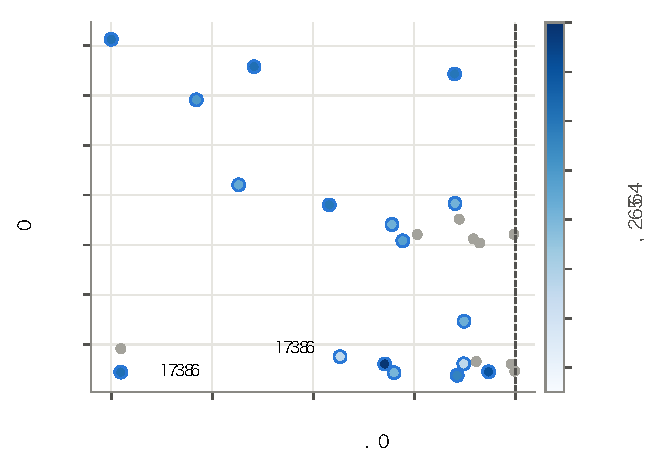
\includegraphics[width=0.62\linewidth]{figs/fig2_pareto.pdf}
\caption{名目シナリオでの事業費–被害額の Pareto 解\prelim（色＝Ecology）。括弧内は Minimax Regret でその案を推奨する主体。}
\label{fig:pareto}
\end{figure}

\begin{table}[h]
\centering\small
\caption{主体ごとの推奨案と最大 Regret\prelim（許容閾値 0.05）}
\label{tab:rdm}
\begin{tabular}{@{}lrrrrrrrr@{}}
\toprule
案（推奨する主体） & 事業費 & 被害額 & 床上世帯 & \multicolumn{4}{c}{最大 Regret} & 最大 $R/\tau$ \\
\cmidrule(lr){5-8}
 & [億円] & [億円] & & 国 & 上流 & 下流 & 住民 & \\
\midrule
施策なし（国） & 0 & 756 & 3,187 & \textbf{0.01} & 0.24 & 0.23 & 0.35 & 7.0 \\
案10（上流自治体） & 631 & 610 & 2,567 & 0.08 & \textbf{0.02} & 0.26 & 0.21 & 5.2 \\
案11（下流自治体） & 1,079 & 590 & 2,336 & 0.19 & 0.33 & \textbf{0.01} & 0.17 & 6.6 \\
案6（住民） & 1,400 & 422 & 1,613 & 0.20 & 0.08 & 0.10 & \textbf{0.01} & 3.9 \\
\textbf{案12（総合推奨）} & 1,133 & 438 & 1,652 & 0.17 & 0.10 & 0.13 & 0.09 & \textbf{3.4} \\
\bottomrule
\end{tabular}

\smallskip
\raggedright\footnotesize
案12：堤防 上流＋1・中流＋1・下流＋2 m、田んぼダム 上流・下流、森林化 下流。
案11：堤防 上流＋2・中流＋1 m、森林化 上流・中流、田んぼダム 下流（事業費の大半が上流・中流に帰着）。
\end{table}

\paragraph{読み取り（想定される記述）}
国は事業費の重み（0.35）が大きいため施策なしを選び、住民は施策の多い案6を選ぶ。
下流自治体の推奨案11は、事業費が主に上流・中流に帰着する（下流の負担 15 億円\prelim）。
このため、上流自治体の最大 Regret が 0.33\prelim と大きい。
すなわち\textbf{対立の主因は費用負担の配分}であり、費用分担ルールを変えれば対立が緩和するかを本計算で検証する（追加実験 E3）。

\begin{figure}[h]
\centering
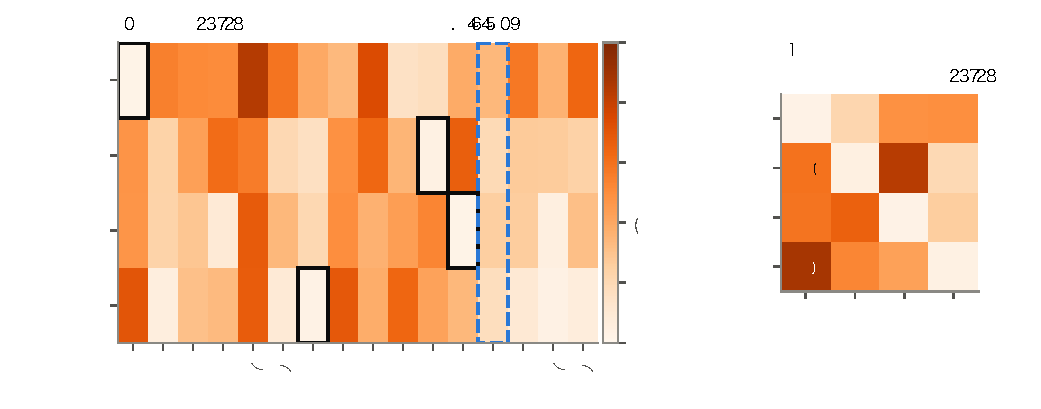
\includegraphics[width=\linewidth]{figs/fig3_regret.pdf}
\caption{(a) Pareto 解ごとの最大 Regret（許容閾値で正規化）\prelim。(b) 列の主体の推奨案を採用したときの、行の主体の最大 Regret（対立）\prelim。}
\label{fig:regret}
\end{figure}

\subsection{不確実性の寄与（RQ2）}
\begin{figure}[h]
\centering
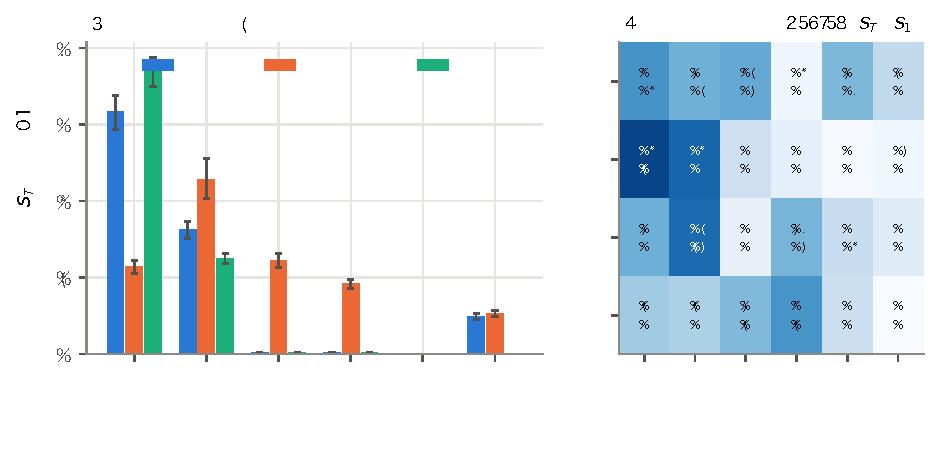
\includegraphics[width=\linewidth]{figs/fig4_sobol.pdf}
\caption{Sobol 指数\prelim。(a) 総合推奨案の被害額・被害軽減額・浸水人口の $S_T$ と 95\% 区間。
(b) 各主体の推奨案の Regret。$S_T\gg S_1$ は相互作用が大きいことを示す。
*浸水人口は代理モデルの誤差が大きく（図\ref{fig:surrogate}）、参考値。}
\label{fig:sobol}
\end{figure}

\paragraph{読み取り} 被害額は降雨倍率と降雨強度分布でほぼ説明される（$S_T$ 0.63, 0.32\prelim）。
一方、被害軽減額（施策の効き）には $\gamma$・田んぼダム効果・降雨倍率・海面上昇が分散して寄与する。
Regret は主体によって支配要因が異なる。上流自治体は降雨倍率・$\gamma$、下流自治体は $\gamma$・海面上昇、
住民は海面上昇・田んぼダム効果である。$S_1$ は小さく、相互作用が支配的である。
Morris では堤防・遊水地・嵩上げの効果係数の感度がほぼ0であった。
堤防については、1000 m では主要河川がわずかな嵩上げで越水しなくなる\textbf{効果の飽和}による
（＋2 m と＋5 m で被害額が同じ）。この点は250 m での確認が必要である（E2）。

\begin{figure}[h]
\centering
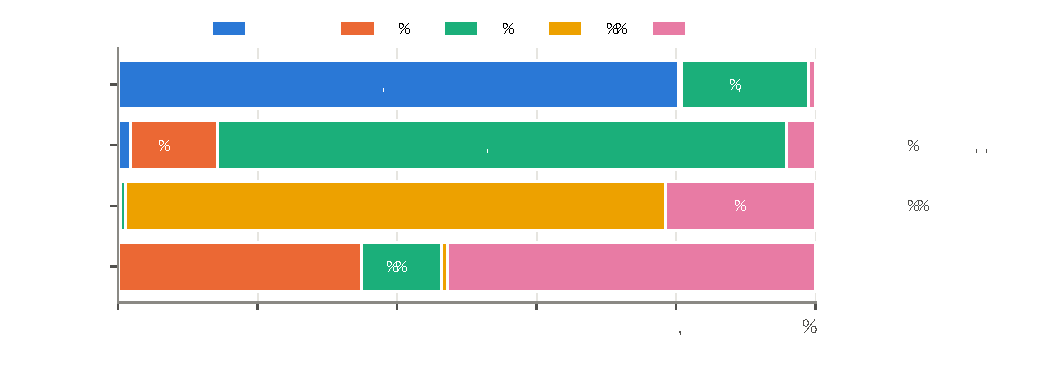
\includegraphics[width=0.9\linewidth]{figs/fig5_decision.pdf}
\caption{意思決定感度\prelim：不確実性パラメータを同時に変えたとき、各主体にとって各案が予算内で最良となる割合。
右は名目最良案（RRI の名目計算）と、そこからの順位逆転率。}
\label{fig:decision}
\end{figure}

\paragraph{読み取り} 国（施策なし 80\%）と下流自治体（案11 77\%）の選択は比較的安定している。
上流自治体は名目最良（案12）と不確実性下の最良（案10, 82\%）が異なる。
住民は案6 と案12 の間で最良案が入れ替わる（53\% / 35\%）。
RQ1 の「名目最適 $\neq$ 頑健」を示す中心の図とする。

\begin{figure}[h]
\centering
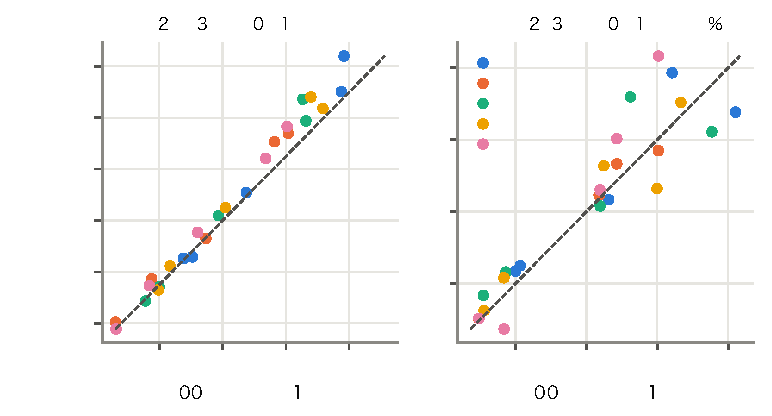
\includegraphics[width=0.75\linewidth]{figs/fig8_surrogate.pdf}
\caption{代理モデルの独立検証（検証 LHS 5点 × 5案）\prelim。被害額は相対 RMSE 6–7\%、
浸水人口は 10–34\%（1000 m ではセルの人口がまとめて閾値を超え、出力が階段状になるため）。}
\label{fig:surrogate}
\end{figure}

\subsection{適応経路（RQ3）}
\begin{figure}[h]
\centering
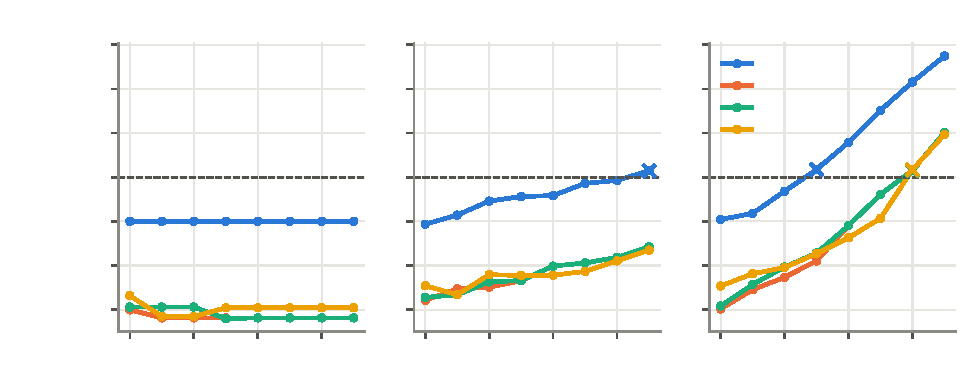
\includegraphics[width=\linewidth]{figs/fig6_dapp_series.pdf}
\caption{代表洪水の被害額（対策なし・現在気候＝1）の推移\prelim。✕＝ATP 到達。}
\label{fig:dappseries}
\end{figure}

\begin{figure}[h]
\centering
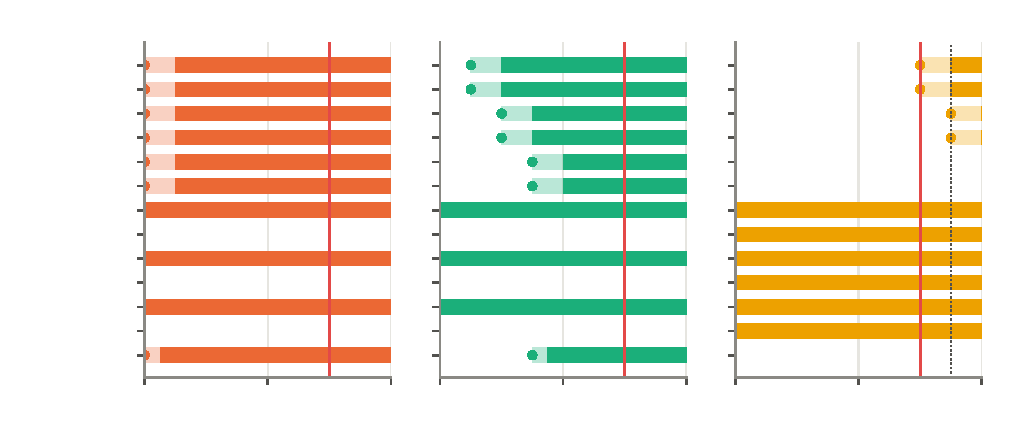
\includegraphics[width=\linewidth]{figs/fig7_pathways.pdf}
\caption{4℃経路での施策の実施\prelim（薄色＝着手〜完成、濃色＝効果あり、点線＝観測による切替、赤線＝ATP）。
論文では Haasnoot 型の Pathways Map（GUI の /dapp）も併記する。}
\label{fig:pathways}
\end{figure}

\begin{table}[h]
\centering\small
\caption{戦略別スコアカード\prelim（累積値は2020年への現在価値、億円）}
\label{tab:dapp}
\begin{tabular}{@{}lrrrrcrrrr@{}}
\toprule
戦略 & \multicolumn{3}{c}{累積期待被害} & 累積費用 & ATP（4℃） & \multicolumn{4}{c}{最大 Regret} \\
\cmidrule(lr){2-4}\cmidrule(lr){7-10}
 & 現在 & 2℃ & 4℃ & & 被害／人口 & 国 & 上流 & 下流 & 住民 \\
\midrule
無対策 & 188 & 199 & 215 & 0 & 2050／2040 & 0.05 & 0.18 & 0.17 & 0.34 \\
早期集中投資 & 108 & 132 & 142 & 1,161 & 2080／2070 & 0.08 & 0.02 & 0.05 & \textbf{0.00} \\
\textbf{段階的投資} & 113 & 133 & 146 & 705 & 2080／2070 & \textbf{0.00} & \textbf{0.01} & 0.02 & 0.01 \\
状況適応型 & 115 & 136 & 152 & 825 & 2080／2070 & 0.03 & 0.05 & \textbf{0.00} & 0.03 \\
\bottomrule
\end{tabular}
\end{table}

\paragraph{読み取り} 段階的投資は、早期集中投資の約6割の費用で、ほぼ同じ被害軽減を得る（総合 Minimax Regret）。
状況適応型は現在気候・2℃では切替が起きず、自然基盤のみで推移する。4℃では2070年代の被害急増を
1期遅れで観測して2080年に堤防に着手するため、完成が ATP に間に合わない（図\ref{fig:pathways}）。
\textbf{観測トリガーの遅れ＋実施遅延}がATP回避を妨げるという結果は、DAPP の signpost 設計への示唆として論文Bの中心に置く。
なお状況適応型の費用のうち約600億円\prelim は森林化による作物収入の損失（維持費扱い）であり、費用の定義に依存する。

%=====================================================================
\section{本計算の計画}
\label{sec:plan}

\begin{table}[H]
\centering\small
\caption{試行と本計算の設定（RRI 1回 約20秒、阿武隈川全域 1000 m）}
\begin{tabularx}{\linewidth}{@{}lllX@{}}
\toprule
項目 & 試行 & 本計算（案） & 備考 \\
\midrule
NSGA-II & 8個体×2世代 & 24個体×10世代 & 収束（ハイパーボリューム）を報告 \\
計算シナリオ & 気候3×1 & 気候3×3以上（LHS） & 気候以外の計算因子を識別するため \\
Morris & 2軌道 & 6軌道以上 & 選別の安定性を確認 \\
代理モデル学習・検証 & 10＋1・5 & 30＋1・8 & 浸水人口の誤差を 15\% 以下に \\
DAPP 戦略 & 4 & 6（自然基盤重視・構造物重視を追加） & 状況適応型のトリガー2種を比較 \\
RRI 回数（概算） & 約240回 & 約800–1,000回（5–6時間） & キャッシュを再利用 \\
\bottomrule
\end{tabularx}
\end{table}

\paragraph{追加実験}
\begin{description}
\item[E1 複数洪水] 代表洪水を複数（他の既往洪水・d4PDF の大雨）にして、推奨案と ATP の変化を調べる。
\item[E2 解像度] 推奨案（施策なし・案10・11・12・6）を250 m で再計算し、順位が保たれるか、堤防効果の飽和が解消するかを確認する。
\item[E3 費用分担] 事業費を便益地域に按分する、または国が一部を負担するルールで、対立（図\ref{fig:regret}b）が緩和するかを調べる。
\item[E4 トリガー] 状況適応型の観測指標を降雨倍率にする、\texttt{monitor\_lag}$=0$、閾値を1.0→0.8にする。
\item[E5 重みの根拠] 自治体・住民への聞き取りやアンケートで重みと許容 Regret を設定し、仮定の重みとの差を示す。
\end{description}

%=====================================================================
\section{想定される査読上の論点と対応}
\label{sec:review}
\begin{table}[H]
\centering\small
\caption{想定される論点と対応}
\begin{tabularx}{\linewidth}{@{}>{\raggedright\arraybackslash}p{42mm}X@{}}
\toprule
論点 & 対応 \\
\midrule
モデルが未校正（流量が過小） & 観測所流量での校正、または水害統計（市町村別）での被害の検証を補足に示す。結論は施策間の\textbf{相対比較}に限る \\
1000 m は粗い & E2（250 m での推奨案の確認）。浸水人口の階段状の挙動を明記する \\
洪水が1イベントのみ & E1。DAPP の「代表洪水×年超過確率」近似と限界（頻度分布・年々変動・連続洪水・頻度変化を表さない）を明記する \\
年超過確率 $p=1/100$ の仮定 & $p$ は期待被害と費用の比を変え、戦略の順位にも影響しうる。$p$ を 1/50〜1/200 で変えた感度を示す \\
重みと許容 Regret が恣意的 & 選好感度（重みのランダム化・掃引）で結論の頑健性を示す。E5 \\
代理モデルの誤差 & 独立検証の誤差を本文に表で示す。浸水人口の感度は参考値として扱う \\
施策効果係数の範囲が仮定 & 根拠／仮定を表で区別し、範囲を広げた感度も示す \\
森林化の費用（作物損失） & 費用の内訳（初期・維持・機会費用）を分けて示す \\
資産・人口が2020年のまま & 社会経済シナリオは今後の課題とする。DAPP では限界として明記する \\
\bottomrule
\end{tabularx}
\end{table}

%=====================================================================
\section{作業計画}
\begin{enumerate}
\item 先行研究の整理と投稿先・本数の決定 \todo{担当・期限}
\item 本計算（RDM → SA → DAPP）と E1–E4
\item 図の確定（本資料の図\ref{fig:pareto}–\ref{fig:pathways}を基本とし、Pathways Map を追加）
\item 論文A執筆 → 共著者確認 → 投稿
\item 論文B執筆（DAPP, E4 を中心に）
\end{enumerate}

\clearpage
\appendix
\section{再現手順}
\begin{verbatim}
.venv/bin/python scripts/run_rdm.py --quick                       # RDM（docs/09）
.venv/bin/python scripts/run_sensitivity.py abukuma_quick --quick # 感度分析（docs/10）
.venv/bin/python scripts/run_dapp.py --quick                      # DAPP（docs/11）
.venv/bin/python docs/paper/make_figs.py                          # 本資料の図
cd docs/paper && latexmk -lualatex paper_plan.tex                 # 本資料
\end{verbatim}
結果：\texttt{data/processed/rdm/abukuma\_quick/}、\texttt{data/processed/dapp/abukuma\_dapp\_quick/}。
各ディレクトリの \texttt{config*.json} に、用いた全設定（不確実性の範囲・根拠・乱数の種）が保存されている。

\end{document}
